\chapter{GLib, the Core Library}
\label{glib}

GLib is the low-level core library that forms the basis for projects such as GTK+ and GNOME. It provides data structures, utility functions, portability wrappers, and other essential functionality such as an event loop and threads. GLib is available on most Unix-like systems and Windows.

This chapter covers some of the most commonly-used features. GLib is simple, and the concepts are familiar; so we'll move quickly. For more complete coverage of GLib, see the latest API documentation that comes with the library (for the development environment, see section~\ref{intro-dev-environment} on p.~\pageref{intro-dev-environment}). By the way: if you have very specific questions about the implementation, don't be afraid to look at the source code. Normally the documentation contains enough information, but if you come across a missing detail, please file a bug (of course, the best would be with a provided patch).

GLib's various facilities are intended to have a consistent interface; the coding style is semi-object-oriented, and identifiers are prefixed with ``g'' to create a kind of namespace.

GLib has a few toplevel headers:
\begin{itemize}
  \item \header{glib.h}, the main header;
  \item \header{gmodule.h} for dynamic loading of modules;
  \item \header{glib-unix.h} for Unix-specific APIs;
  \item \header{glib/gi18n.h} and \header{glib/gi18n-lib.h} for internationalization;
  \item \header{glib/gprintf.h} and \header{glib/gstdio.h} to avoid pulling in all of stdio.
\end{itemize}

\bigskip
Note: instead of reinventing the wheel, this chapter is heavily based on the corresponding chapter in the book \emph{GTK+/Gnome Application Development} by Havoc Pennington, licensed under the Open Publication License (see section~\ref{intro-license} p.~\pageref{intro-license}). GLib has a very stable API. Despite the fact that Havoc Pennington's book was written in 1999 (for GLib~1.2), only a few updates were required to fit the latest GLib versions (version~2.42 at the time of writing).

\section{Basics}

GLib provides substitutes for many standard and commonly-used C language constructs. This section describes GLib's fundamental type definitions, macros, memory allocation routines, and string utility functions.

\subsection{Type Definitions}

Rather than using C's standard types (\lstinline{int}, \lstinline{long}, etc.) GLib defines its own. These serve a variety of purposes. For example, \lstinline{gint32} is guaranteed to be 32 bits wide, something no standard C89 type can ensure. \lstinline{guint} is simply easier to type than \lstinline{unsigned}. A few of the typedefs exist only for consistency; for example, \lstinline{gchar} is always equivalent to the standard \lstinline{char}.

The most important primitive types defined by GLib:
\begin{itemize}
  \item \lstinline{gint8}, \lstinline{guint8}, \lstinline{gint16}, \lstinline{guint16}, \lstinline{gint32}, \lstinline{guint32}, \lstinline{gint64}, \lstinline{guint64} --- these give you integers of a guaranteed size. (If it isn't obvious, the \lstinline{guint} types are unsigned, the \lstinline{gint} types are signed.)

  \item \lstinline{gboolean} is useful to make your code more readable, since C89 has no \lstinline{bool} type.

  \item \lstinline{gchar}, \lstinline{gshort}, \lstinline{glong}, \lstinline{gint}, \lstinline{gfloat}, \lstinline{gdouble} are purely cosmetic.

  \item \lstinline{gpointer} may be more convenient to type than \lstinline{void *}. \lstinline{gconstpointer} gives you \lstinline{const void *}. (\lstinline{const gpointer} will \emph{not} do what you typically mean it to; spend some time with a good book on C if you don't see why.)

  \item \lstinline{gsize} is an unsigned integer type that can hold the result of the \lstinline{sizeof} operator.
\end{itemize}

\subsection{Frequently Used Macros}

GLib defines a number of familiar macros used in many C programs, shown in Listing~\ref{glib-simplemacros}. All of these should be self-explanatory. \lstinline{MIN()}/\lstinline{MAX()} return the smaller or larger of their arguments. \lstinline{ABS()} returns the absolute value of its argument. \lstinline{CLAMP(x, low, high)} means \lstinline{x}, unless \lstinline{x} is outside the range [\lstinline{low},~\lstinline{high}]; if \lstinline{x} is below the range, \lstinline{low} is returned; if \lstinline{x} is above the range, \lstinline{high} is returned. In addition to the macros shown in Listing~\ref{glib-simplemacros}, \lstinline{TRUE}/\lstinline{FALSE}/\lstinline{NULL} are defined as the usual \lstinline{1}/\lstinline{0}/\lstinline{((void *)0)}.

\begin{lstlisting}[float, caption={Familiar C Macros}, label=glib-simplemacros]
#include <glib.h>

MAX (a, b);
MIN (a, b);
ABS (x);
CLAMP (x, low, high);
\end{lstlisting}

There are also many macros unique to GLib, such as the portable \lstinline{gpointer}-to-\lstinline{gint} and \lstinline{gpointer}-to-\lstinline{guint} conversions shown in Listing~\ref{glib-pointerint}.

\begin{lstlisting}[float, caption={Macros for storing integers in pointers}, label=glib-pointerint]
#include <glib.h>

GINT_TO_POINTER (p);
GPOINTER_TO_INT (p);
GUINT_TO_POINTER (p);
GPOINTER_TO_UINT (p);
\end{lstlisting}

Most of GLib's data structures are designed to store a \lstinline{gpointer}. If you want to store pointers to dynamically allocated objects, this is the right thing. However, sometimes you want to store a simple list of integers without having to dynamically allocate them. Though the C standard does not strictly guarantee it, it is possible to store a \lstinline{gint} or \lstinline{guint} in a \lstinline{gpointer} variable on the wide range of platforms GLib has been ported to; in some cases, an intermediate cast is required. The macros in Listing~\ref{glib-pointerint} abstract the presence of the cast.

Here's an example:
\begin{lstlisting}
gint my_int;
gpointer my_pointer;

my_int = 5;
my_pointer = GINT_TO_POINTER (my_int);
printf ("We are storing %d\n", GPOINTER_TO_INT (my_pointer));
\end{lstlisting}

Be careful, though; these macros allow you to store an integer in a pointer, but storing a pointer in an integer will \emph{not} work. To do that portably, you must store the pointer in a \lstinline{long}. (It's undoubtedly a bad idea to do so, however.)

\subsection{Debugging Macros}

GLib has a nice set of macros you can use to enforce invariants and preconditions in your code. GTK+ uses these liberally -- one of the reasons it's so stable and easy to use. They all disappear when you define \lstinline{G_DISABLE_CHECKS} or \lstinline{G_DISABLE_ASSERT}, so there's no performance penalty in production code. Using these liberally is a very, very good idea. You'll find bugs much faster if you do. You can even add assertions and checks whenever you find a bug to be sure the bug doesn't reappear in future versions -- this complements a regression suite. Checks are especially useful when the code you're writing will be used as a black box by other programmers; users will immediately know when and how they've misused your code.

Of course you should be very careful to ensure your code isn't subtly dependent on debug-only statements to function correctly. Statements that will disappear in production code should \emph{never} have side effects.

\begin{lstlisting}[float, caption={Precondition Checks}, label=glib-precondition]
#include <glib.h>

g_return_if_fail (condition);
g_return_val_if_fail (condition, return_value);
\end{lstlisting}

%TODO add gobject chapter reference when the chapter is written
Listing~\ref{glib-precondition} shows GLib's precondition checks. \lstinline{g_return_if_fail()} prints a warning and immediately returns from the current function if \lstinline{condition} is \lstinline{FALSE}. \lstinline{g_return_val_if_fail()} is similar but allows you to return some \lstinline{return_value}. These macros are incredibly useful -- if you use them liberally, especially in combination with GObject's runtime type checking, %(see chapter~\ref{gobject})
you'll halve the time you spend looking for bad pointers and type errors.

Using these functions is simple; here's an example from the GLib hash table implementation:
\begin{lstlisting}
void
g_hash_table_foreach (GHashTable *hash_table,
                      GHFunc      func,
                      gpointer    user_data)
{
  gint i;

  g_return_if_fail (hash_table != NULL);
  g_return_if_fail (func != NULL);

  for (i = 0; i < hash_table->size; i++)
    {
      guint node_hash = hash_table->hashes[i];
      gpointer node_key = hash_table->keys[i];
      gpointer node_value = hash_table->values[i];

      if (HASH_IS_REAL (node_hash))
        (* func) (node_key, node_value, user_data);
    }
}
\end{lstlisting}

Without the checks, passing \lstinline{NULL} as a parameter to this function would result in a mysterious segmentation fault. The person using the library would have to figure out where the error occurred with a debugger, and maybe even dig in to the GLib code to see what was wrong. With the checks, they'll get a nice error message telling them that \lstinline{NULL} arguments are not allowed.

\begin{lstlisting}[float, caption={Assertions}, label=glib-assertions]
#include <glib.h>

g_assert (condition);
g_assert_not_reached ();
\end{lstlisting}

GLib also has more traditional assertion macros, shown in Listing~\ref{glib-assertions}. \lstinline{g_assert()} is basically identical to \lstinline{assert()}, but responds to \lstinline{G_DISABLE_ASSERT} and behaves consistently across all platforms. \lstinline{g_assert_not_reached()} is also provided; this is an assertion which always fails. Assertions call \lstinline{abort()} to exit the program and (if your environment supports it) dump a core file for debugging purposes.

Fatal assertions should be used to check \emph{internal consistency} of a function or library, while \lstinline{g_return_if_fail()} is intended to ensure sane values are passed to the public interfaces of a program module. That is, if an assertion fails, you typically look for a bug in the module containing the assertion; if a \lstinline{g_return_if_fail()} check fails, you typically look for the bug in the code which invokes the module.

This code from GLib's calendrical calculations module shows the difference:
\begin{lstlisting}
GDate *
g_date_new_dmy (GDateDay   day,
                GDateMonth month,
                GDateYear  year)
{
  GDate *date;
  g_return_val_if_fail (g_date_valid_dmy (day, month, year), NULL);

  date = g_new (GDate, 1);

  date->julian = FALSE;
  date->dmy = TRUE;

  date->month = month;
  date->day = day;
  date->year = year;

  g_assert (g_date_valid (date));

  return date;
}
\end{lstlisting}

The precondition check at the beginning ensures the user passes in reasonable values for the day, month and year; the assertion at the end ensures that GLib constructed a sane object, given sane values.

\lstinline{g_assert_not_reached()} should be used to mark ``impossible'' situations; a common use is to detect switch statements that don't handle all possible values of an enumeration:
\begin{lstlisting}
switch (value)
  {
  case FOO_ONE:
    break;

  case FOO_TWO:
    break;

  default:
    g_assert_not_reached ();
  }
\end{lstlisting}

All of the debugging macros print a warning using GLib's \lstinline{g_log()} facility, which means the warning includes the name of the originating application or library, and you can optionally install a replacement warning-printing routine. For example, you might send all warnings to a dialog box or log file instead of printing them on the console.

\subsection{Memory}

GLib wraps the standard \lstinline{malloc()} and \lstinline{free()} with its own \lstinline{g_} variants, \lstinline{g_malloc()} and \lstinline{g_free()}, shown in Listing~\ref{glib-malloc-free}.
These are nice in several small ways:

\begin{itemize}
  \item \lstinline{g_malloc()} always returns a \lstinline{gpointer}, never a \lstinline{char *}, so there's no need to cast the return value.

  \item \lstinline{g_malloc()} aborts the program if the underlying \lstinline{malloc()} fails, so you don't have to check for a \lstinline{NULL} return value.

  \item \lstinline{g_malloc()} gracefully handles a \lstinline{size} of \lstinline{0}, by returning \lstinline{NULL}.

  \item \lstinline{g_free()} will ignore any \lstinline{NULL} pointers you pass to it.
\end{itemize}

\begin{lstlisting}[float, caption={GLib memory allocation}, label=glib-malloc-free]
#include <glib.h>

gpointer g_malloc (gsize n_bytes);
void g_free (gpointer mem);
gpointer g_realloc (gpointer mem, gsize n_bytes);
gpointer g_memdup (gconstpointer mem, guint n_bytes);
\end{lstlisting}

It's important to match \lstinline{g_malloc()} with \lstinline{g_free()}, plain \lstinline{malloc()} with \lstinline{free()}, and (if you're using C++) \lstinline[language=C++]{new} with \lstinline[language=C++]{delete}. Otherwise bad things can happen, since these allocators may use different memory pools (and \lstinline[language=C++]{new}/\lstinline[language=C++]{delete} call constructors and destructors).

Of course there's a \lstinline{g_realloc()} equivalent to \lstinline{realloc()}. There's also a convenient \lstinline{g_malloc0()} which fills allocated memory with 0s, and \lstinline{g_memdup()} which returns a copy of \lstinline{n_bytes} bytes starting at \lstinline{mem}. \lstinline{g_realloc()} and \lstinline{g_malloc0()} will both accept a size of 0, for consistency with \lstinline{g_malloc()}. However, \lstinline{g_memdup()} will not.

%TODO mention this in the API doc
If it isn't obvious: \lstinline{g_malloc0()} fills raw memory with unset bits, not the value 0 for whatever type you intend to put there. Occasionally someone expects to get an array of floating point numbers initialized to 0.0; this is \emph{not} guaranteed to work portably.

Finally, there are type-aware allocation macros, shown in Listing~\ref{glib-g_new}. The \lstinline{type} argument to each of these is the name of a type, and the \lstinline{count} argument is the number of \lstinline{type}-size blocks to allocate. These macros save you some typing and multiplication, and are thus less error-prone. They automatically cast to the target pointer type, so attempting to assign the allocated memory to the wrong kind of pointer should trigger a compiler warning. (If you have warnings turned on, as a responsible programmer should!)

\begin{lstlisting}[float, caption={Allocation macros}, label=glib-g_new]
#include <glib.h>

g_new (type, count);
g_new0 (type, count);
g_renew (type, mem, count);
\end{lstlisting}

\subsection{String Handling}

GLib provides a number of functions for string handling; some are unique to GLib, and some solve portability concerns. They all interoperate nicely with the GLib memory allocation routines.

For those interested in a better string than \lstinline{gchar *}, there's also a \lstinline{GString} type. It isn't covered in this book, see the API documentation for further information.

\begin{lstlisting}[float, caption={Portability Wrapper}, label=glib-strext]
gint g_snprintf (gchar *string, gulong n, gchar const *format, ...);
\end{lstlisting}

Listing~\ref{glib-strext} shows a substitute GLib provides for the \lstinline{snprintf()} function. \lstinline{g_snprintf()} wraps native \lstinline{snprintf()} on platforms that have it, and provides an implementation on those that don't.

Pay attention to not use the crash-causing, security-hole-creating, generally evil \lstinline{sprintf()} function. By using the relatively safe \lstinline{g_snprintf()} or \lstinline{g_strdup_printf()} (see below), you can say goodbye to \lstinline{sprintf()} forever.

\begin{lstlisting}[float, caption={Allocating Strings}, label=glib-strdup]
#include <glib.h>

gchar * g_strdup (const gchar *str);
gchar * g_strndup (const gchar *str, gsize n);
gchar * g_strdup_printf (const gchar *format, ...);
gchar * g_strdup_vprintf (const gchar *format, va_list args);
gchar * g_strnfill (gsize length, gchar fill_char);
\end{lstlisting}

Listing~\ref{glib-strdup} shows GLib's rich array of functions for allocating strings. Unsurprisingly, \lstinline{g_strdup()} and \lstinline{g_strndup()} produce an allocated copy of \lstinline{str} or the first \lstinline{n} characters of \lstinline{str}. For consistency with the GLib memory allocation functions, they return \lstinline{NULL} if passed a \lstinline{NULL} pointer. The \lstinline{printf()} variants return a formatted string. \lstinline{g_strnfill()} returns a string of size \lstinline{length} filled with \lstinline{fill_char}.

\lstinline{g_strdup_printf()} deserves a special mention; it is a simpler way to handle this common piece of code:
\begin{lstlisting}
gchar *str = g_malloc (256);
g_snprintf (str, 256, "%d printf-style %s", num, string);
\end{lstlisting}

Instead you could say this, and avoid having to figure out the proper length of the buffer to boot:
\begin{lstlisting}
gchar *str = g_strdup_printf ("%d printf-style %s", num, string);
\end{lstlisting}

\begin{lstlisting}[float, caption={In-place string modifications}, label=glib-strmanip]
#include <glib.h>

gchar * g_strchug (gchar *string);
gchar * g_strchomp (gchar *string);
gchar * g_strstrip (gchar *string);
\end{lstlisting}

The functions in Listing~\ref{glib-strmanip} modify a string in-place: \lstinline{g_strchug()} and \lstinline{g_strchomp()} ``chug'' the string (remove leading spaces), or ``chomp'' it (remove trailing spaces). Those two functions return the string, in addition to modifying it in-place; in some cases it may be convenient to use the return value. There is a macro, \lstinline{g_strstrip()}, which combines both functions to remove both leading and trailing spaces.

\begin{lstlisting}[float, caption={String Conversions}, label=glib-strformats]
#include <glib.h>

gdouble g_strtod (const gchar *nptr, gchar **endptr);
const gchar * g_strerror (gint errnum);
const gchar * g_strsignal (gint signum);
\end{lstlisting}

Listing~\ref{glib-strformats} shows a few more semi-standard functions GLib wraps. \lstinline{g_strtod} is like \lstinline{strtod()} -- it converts string \lstinline{nptr} to a double -- with the exception that it will also attempt to convert the double in the \texttt{"C"} locale if it fails to convert it in the user's default locale. \lstinline{*endptr} is set to the first unconverted character, i.e. any text after the number representation. If conversion fails, \lstinline{*endptr} is set to \lstinline{nptr}. \lstinline{endptr} may be \lstinline{NULL}, causing it to be ignored.

\lstinline{g_strerror()} and \lstinline{g_strsignal()} are like their non-\lstinline{g_} equivalents, but portable. (They return a string representation for an \lstinline{errno} or a signal number.)

\begin{lstlisting}[float, caption={Concatenating Strings}, label=glib-strconcat]
#include <glib.h>

gchar * g_strconcat (const gchar *string1, ...);
gchar * g_strjoin (const gchar *separator, ...);
\end{lstlisting}

GLib provides some convenient functions for concatenating strings, shown in Listing~\ref{glib-strconcat}. \lstinline{g_strconcat()} returns a newly-allocated string created by concatenating each of the strings in the argument list. The last argument must be \lstinline{NULL}, so \lstinline{g_strconcat()} knows when to stop. \lstinline{g_strjoin()} is similar, but \lstinline{separator} is inserted between each string. If \lstinline{separator} is \lstinline{NULL}, no separator is used.

\begin{lstlisting}[float, caption={Manipulating \lstinline{NULL}-terminated string vectors}, label=glib-strvector]
#include <glib.h>

gchar ** g_strsplit (const gchar *string,
                     const gchar *delimiter,
                     gint max_tokens);
gchar * g_strjoinv (const gchar *separator, gchar **str_array);
void g_strfreev (gchar **str_array);
\end{lstlisting}

Finally, Listing~\ref{glib-strvector} summarizes a few routines which manipulate \lstinline{NULL}-terminated arrays of strings. \lstinline{g_strsplit()} breaks \lstinline{string} at each \lstinline{delimiter}, returning a newly-allocated array. \lstinline{g_strjoinv()} concatenates each string in the array with an optional \lstinline{separator}, returning an allocated string. \lstinline{g_strfreev()} frees each string in the array and then the array itself.

\section{Data Structures}

GLib implements many common data structures, so you don't have to reinvent the wheel every time you want a linked list. This section covers GLib's implementation of linked lists, sorted binary trees, N-ary trees, and hash tables.

\subsection{Lists}

GLib provides generic single and doubly linked lists, \lstinline{GSList} and \lstinline{GList}, respectively. These are implemented as lists of \lstinline{gpointer}; you can use them to hold integers with the \lstinline{GINT_TO_POINTER} and \lstinline{GPOINTER_TO_INT} macros. \lstinline{GSList} and \lstinline{GList} have almost the same API's, except that there is a \lstinline{g_list_previous()} function and no \lstinline{g_slist_previous()}. This section will discuss \lstinline{GSList} but everything also applies to the doubly linked list.

\begin{lstlisting}[float, caption={\lstinline{GSList} cell}, label=glib-gslist-cell]
typedef struct _GSList GSList;

struct _GSList
{
  gpointer data;
  GSList *next;
};
\end{lstlisting}

A \lstinline{GSList} cell is a self-explanatory structure shown in Listing~\ref{glib-gslist-cell}. The structure fields are public, so you can use them directly to access the data or to traverse the list.

In the GLib implementation, the empty list is simply a \lstinline{NULL} pointer. It's always safe to pass \lstinline{NULL} to list functions since it's a valid list of length 0. Code to create a list and add one element might look like this:
\begin{lstlisting}
GSList *list = NULL;
gchar *element = g_strdup ("a string");
list = g_slist_append (list, element);
\end{lstlisting}

GLib lists have a noticeable Lisp influence; the empty list is a special ``nil'' value for that reason. \lstinline{g_slist_prepend()} works much like \texttt{cons} -- it's a constant-time operation ($O(1)$) that adds a new cell to the front of the list.

\begin{lstlisting}[float, caption={Changing linked list contents}, label=glib-listchanging]
#include <glib.h>

GSList * g_slist_append (GSList *list, gpointer data);
GSList * g_slist_prepend (GSList *list, gpointer data);
GSList * g_slist_insert (GSList *list, gpointer data, gint position);
GSList * g_slist_remove (GSList *list, gconstpointer data);
\end{lstlisting}

Listing~\ref{glib-listchanging} shows the basic functions for changing \lstinline{GSList} contents. For all of these, you must assign the return value to your list pointer in case the head of the list changes. Note that GLib does \emph{not} store a pointer to the tail of the list, so the append, insert, and remove functions run in $O(n)$ time, with $n$ the length of the list.

GLib will handle memory issues, deallocating and allocating list cells as needed. For example, the following code would remove the above-added element and empty the list:
\begin{lstlisting}
list = g_slist_remove (list, element);
\end{lstlisting}

\lstinline{list} is now \lstinline{NULL}. You still have to free \lstinline{element} yourself, of course.

To access a list element, you refer to the \lstinline{GSList} struct directly:
\begin{lstlisting}
gchar *my_data = list->data;
\end{lstlisting}

To iterate over the list, you might write code like this:
\begin{lstlisting}
GSList *l;

for (l = list; l != NULL; l = l->next)
  {
    gchar *str = l->data;
    g_print ("Element: %s\n", str);
  }
\end{lstlisting}

\begin{lstlisting}[float, caption={Freeing entire linked lists}, label=glib-listfree]
#include <glib.h>

typedef void (* GDestroyNotify) (gpointer data);

void g_slist_free (GSList *list);
void g_slist_free_full (GSList *list, GDestroyNotify free_func);
\end{lstlisting}

Listing~\ref{glib-listfree} shows functions to clear an entire list. \lstinline{g_slist_free()} removes all the links in one fell swoop. \lstinline{g_slist_free()} has no return value because it would always be \lstinline{NULL}, and you can simply assign that value to your list if you like. Obviously, \lstinline{g_slist_free()} frees only the list cells; it has no way of knowing what to do with the list contents. The smarter function \lstinline{g_slist_free_full()} takes a second argument with a destroy function pointer that is called on each element's data. To free the list containing dynamically-allocated strings, you can write:
\begin{lstlisting}
g_slist_free_full (list, g_free);

/* If list may be used later: */
list = NULL;
\end{lstlisting}

This is equivalent of writing:
\begin{lstlisting}
GSList *l;

for (l = list; l != NULL; l = l->next)
  g_free (l->data);

g_slist_free (list);
list = NULL;
\end{lstlisting}

Constructing a list using \lstinline{g_slist_append()} is a \emph{terrible} idea; use \lstinline{g_slist_prepend()} and then call \lstinline{g_slist_reverse()} if you need items in a particular order. If you anticipate frequently appending to a list, you can also keep a pointer to the last element. The following code can be used to perform efficient appends\footnote{A more convenient way is to use the \lstinline{GQueue} data type: a double-ended queue that keeps a pointer to the head, a pointer to the tail, and the length of the doubly linked list.}:

\pagebreak[2]
\begin{lstlisting}
void
efficient_append (GSList   **list,
                  GSList   **list_end,
                  gpointer   data)
{
  g_return_if_fail (list != NULL);
  g_return_if_fail (list_end != NULL);

  if (*list == NULL)
    {
      g_assert (*list_end == NULL);

      *list = g_slist_append (*list, data);
      *list_end = *list;
    }
  else
    {
      *list_end = g_slist_append (*list_end, data)->next;
    }
}
\end{lstlisting}

To use this function, you would store the list and its end somewhere, and pass their address to \lstinline{efficient_append()}:
\begin{lstlisting}
GSList* list = NULL;
GSList* list_end = NULL;

efficient_append (&list, &list_end, g_strdup ("Foo"));
efficient_append (&list, &list_end, g_strdup ("Bar"));
efficient_append (&list, &list_end, g_strdup ("Baz"));
\end{lstlisting}

Of course you have to be careful not to use any list functions that might change the end of the list without updating \lstinline{list_end}.

\begin{lstlisting}[float, caption={Accessing data in a linked list}, label=glib-listaccess]
#include <glib.h>

typedef void (* GFunc) (gpointer data, gpointer user_data);

GSList * g_slist_find (GSList *list, gconstpointer data);
GSList * g_slist_nth (GSList *list, guint n);
gpointer g_slist_nth_data (GSList *list, guint n);
GSList * g_slist_last (GSList *list);
gint g_slist_index (GSList *list, gconstpointer data);
void g_slist_foreach (GSList *list, GFunc func, gpointer user_data);
\end{lstlisting}

For accessing list elements, the functions in Listing~\ref{glib-listaccess} are provided. None of these change the list's structure. \lstinline{g_slist_foreach()} applies a \lstinline{GFunc} to each element of the list.

Used in \lstinline{g_slist_foreach()}, your \lstinline{GFunc} will be called on each \lstinline{list->data} in \lstinline{list}, passing the \lstinline{user_data} you provided to \lstinline{g_slist_foreach()}. \lstinline{g_slist_foreach()} is comparable to Scheme's ``map'' function.

For example, you might have a list of strings, and you might want to be able to create a parallel list with some transformation applied to the strings. Here is some code, using the \lstinline{efficient_append()} function from an earlier example:

\begin{lstlisting}
typedef struct _AppendContext AppendContext;
struct _AppendContext
{
  GSList *list;
  GSList *list_end;
  const gchar *append;
};

static void
append_foreach (gpointer data,
                gpointer user_data)
{
  gchar *oldstring = data;
  AppendContext *context = user_data;

  efficient_append (&context->list,
                    &context->list_end,
                    g_strconcat (oldstring, context->append, NULL));
}

GSList *
copy_with_append (GSList      *list_of_strings,
                  const gchar *append)
{
  AppendContext context;

  context.list = NULL;
  context.list_end = NULL;
  context.append = append;

  g_slist_foreach (list_of_strings, append_foreach, &context);

  return context.list;
}
\end{lstlisting}

GLib and GTK+ use the ``function pointer and user data'' idiom heavily. If you have functional programming experience, this  is much like using lambda expressions to create a \emph{closure}. (A closure combines a function with an \emph{environment} -- a set of name-value bindings. In this case the ``environment'' is the user data you pass to \lstinline{append_foreach()}, and the ``closure'' is the combination of the function pointer and the user data.)

\begin{lstlisting}[float, caption={Manipulating a linked list}, label=glib-listmanip]
#include <glib.h>

guint g_slist_length (GSList *list);
GSList * g_slist_concat (GSList *list1, GSList *list2);
GSList * g_slist_reverse (GSList *list);
GSList * g_slist_copy (GSList *list);
\end{lstlisting}

There are some handy list-manipulation routines, listed in Listing~\ref{glib-listmanip}. With the exception of \lstinline{g_slist_copy()}, all of these affect the lists in-place. Which means you must assign the return value and forget about the passed-in pointer, just as you do when adding or removing list elements. \lstinline{g_slist_copy()} returns a newly-allocated list, so you can continue to use both lists and must free both lists eventually.

\begin{lstlisting}[float, caption={Sorted lists}, label=glib-listsorted]
#include <glib.h>

typedef gint (* GCompareFunc) (gconstpointer a, gconstpointer b);

GSList * g_slist_insert_sorted (GSList *list, gpointer data, GCompareFunc func);
GSList * g_slist_sort (GSList *list, GCompareFunc compare_func);
GSList * g_slist_find_custom (GSList *list, gconstpointer data, GCompareFunc func);
\end{lstlisting}

Finally, there are some provisions for sorted lists, shown in Listing~\ref{glib-listsorted}. To use these, you must write a \lstinline{GCompareFunc}, which is just like the comparison function in the standard C \lstinline{qsort()}.

If \lstinline{a < b}, the \lstinline{GCompareFunc} should return a negative value; if \lstinline{a > b} a positive value; if \lstinline{a == b} it should return 0.

Once you have a comparison function, you can insert an element into an already-sorted list, or sort an entire list. Lists are sorted in ascending order. You can even recycle your \lstinline{GCompareFunc} to find list elements, using \lstinline{g_slist_find_custom()}.

Be careful with sorted lists; misusing them can rapidly become very inefficient. For example, \lstinline{g_slist_insert_sorted()} is an $O(n)$ operation, but if you use it in a loop to insert multiple elements the loop runs in quadratic time ($O(n^2)$). It's better to simply prepend all your elements, and then call \lstinline{g_slist_sort()}. \lstinline{g_slist_sort()} runs in $O(n \log n)$.

You can also use the \lstinline{GSequence} data structure for sorted data. \lstinline{GSequence} has an API of a list, but is implemented internally with a balanced binary tree.

\subsection{Trees}

There are two different kinds of tree in GLib; \lstinline{GTree} is your basic balanced binary tree, useful to store key-value pairs sorted by key; \lstinline{GNode} stores arbitrary tree-structured data, such as a parse tree or taxonomy.

\subsubsection{GTree}

%FIXME talk about g_tree_ref() and g_tree_unref()? Those functions are often better than g_tree_destroy(), but it needs a bit of explanation on memory management with reference counting. The same applies for GHashTable.
\begin{lstlisting}[float, caption={Creating and destroying balanced binary trees}, label=glib-treeconstruct]
#include <glib.h>

typedef gint (* GCompareFunc) (gconstpointer a, gconstpointer b);
typedef gint (* GCompareDataFunc) (gconstpointer a,
                                   gconstpointer b,
                                   gpointer user_data);

GTree * g_tree_new (GCompareFunc key_compare_func);

GTree * g_tree_new_full (GCompareDataFunc key_compare_func,
                         gpointer key_compare_data,
                         GDestroyNotify key_destroy_func,
                         GDestroyNotify value_destroy_func);

void g_tree_destroy (GTree *tree);
\end{lstlisting}

To create and destroy a \lstinline{GTree}, use a constructor and destructor displayed in Listing~\ref{glib-treeconstruct}. \lstinline{GCompareFunc} is the same \lstinline{qsort()}-style comparison function described for \lstinline{GSList}; in this case it's used to compare keys in the tree. \lstinline{g_tree_new_full()} is useful to ease memory management for dynamically-allocated keys and values.

The \lstinline{GTree} struct is an opaque data type. Its content is accessed and modified only with public functions.

\begin{lstlisting}[float, caption={Manipulating \lstinline{GTree} contents}, label=glib-treemanip]
#include <glib.h>

void g_tree_insert (GTree *tree, gpointer key, gpointer value);
gboolean g_tree_remove (GTree *tree, gconstpointer key);
gpointer g_tree_lookup (GTree *tree, gconstpointer key);
\end{lstlisting}

Functions for manipulating the contents of the tree are shown in Listing~\ref{glib-treemanip}. All very straightforward; \lstinline{g_tree_insert()} overwrites any existing value, so if you don't use \lstinline{g_tree_new_full()}, be careful if the existing value is your only pointer to a chunk of allocated memory. If \lstinline{g_tree_lookup()} fails to find the key, it returns \lstinline{NULL}, otherwise it returns the associated value. Both keys and values have type \lstinline{gpointer} or \lstinline{gconstpointer}, but the \lstinline{GPOINTER_TO_INT()} and \lstinline{GPOINTER_TO_UINT()} macros allow you to use integers instead.

\begin{lstlisting}[float, caption={Determining the size of a \lstinline{GTree}}, label=glib-treesize]
#include <glib.h>

gint g_tree_nnodes (GTree *tree);
gint g_tree_height (GTree *tree);
\end{lstlisting}

There are two functions which give you an idea how large the tree is, shown in Listing~\ref{glib-treesize}.

\begin{lstlisting}[float, caption={Traversing a \lstinline{GTree}}, label=glib-treetraverse]
#include <glib.h>

typedef gboolean (* GTraverseFunc) (gpointer key,
                                    gpointer value,
                                    gpointer data);

void g_tree_foreach (GTree *tree, GTraverseFunc func, gpointer user_data);
\end{lstlisting}

Using \lstinline{g_tree_foreach()} (Listing~\ref{glib-treetraverse}) you can walk the entire tree. To use it, you provide a \lstinline{GTraverseFunc}, which is passed each key-value pair and a \lstinline{data} argument you give to \lstinline{g_tree_foreach()}. Traversal continues as long as the \lstinline{GTraverseFunc} returns \lstinline{FALSE}; if it ever returns \lstinline{TRUE} then traversal stops. You can use this to search the tree by \emph{value}.

\subsubsection{GNode}

\begin{lstlisting}[float, caption={\lstinline{GNode} cell}, label=glib-nodecell]
typedef struct _GNode GNode;

struct _GNode
{
  gpointer data;
  GNode *next;
  GNode *prev;
  GNode *parent;
  GNode *children;
};
\end{lstlisting}

A \lstinline{GNode} is an N-ary tree, implemented as a doubly linked list with parent and child lists. Thus, most list operations have analogues in the \lstinline{GNode} API. You can walk the tree in various ways. Listing~\ref{glib-nodecell} shows the declaration for a node.

\begin{lstlisting}[float, caption={Accessing \lstinline{GNode}}, label=glib-nodeaccess]
#include <glib.h>

g_node_prev_sibling (node);
g_node_next_sibling (node);
g_node_first_child (node);
\end{lstlisting}

There are macros to access \lstinline{GNode} members, shown in Listing~\ref{glib-nodeaccess}. As with \lstinline{GList}, the \lstinline{data} member is intended to be used directly. These macros return the \lstinline{next}, \lstinline{prev}, and \lstinline{children} members respectively; they also check whether their argument is \lstinline{NULL} before dereferencing it, and return \lstinline{NULL} if it is.

\begin{lstlisting}[float, caption={Creating a \lstinline{GNode}}, label=glib-nodenew]
#include <glib.h>

GNode * g_node_new (gpointer data);
\end{lstlisting}

To create a node, the usual \lstinline{_new()} function is provided (Listing~\ref{glib-nodenew}). \lstinline{g_node_new()} creates a childless and parentless node containing \lstinline{data}. Typically \lstinline{g_node_new()} is used only to create the root node; convenience macros are provided which automatically create new nodes as needed.

\begin{lstlisting}[float, caption={Building a \lstinline{GNode} tree}, label=glib-nodebuild]
#include <glib.h>

GNode * g_node_insert (GNode *parent, gint position, GNode *node);
GNode * g_node_insert_before (GNode *parent, GNode *sibling, GNode *node);
GNode * g_node_prepend (GNode *parent, GNode *node);
\end{lstlisting}

To build a tree the fundamental operations shown in Listing~\ref{glib-nodebuild} are used. Each operation returns the just-added node, for convenience when writing loops or recursing the tree. Unlike \lstinline{GList}, it is safe to ignore the return value.

\begin{lstlisting}[float, caption={Building a \lstinline{GNode}}, label=glib-nodeconv]
#include <glib.h>

g_node_append (parent, node);
g_node_insert_data (parent, position, data);
g_node_insert_data_before (parent, sibling, data);
g_node_prepend_data (parent, data);
g_node_append_data (parent, data);
\end{lstlisting}

The convenience macros shown in Listing~\ref{glib-nodeconv} are implemented in terms of the fundamental operations. \lstinline{g_node_append()} is analagous to \lstinline{g_node_prepend()}; the rest take a \lstinline{data} argument, automatically allocate a node for it, and call the corresponding basic operation.

\begin{lstlisting}[float, caption={Destroying a \lstinline{GNode}}, label=glib-nodedestroy]
#include <glib.h>

void g_node_destroy (GNode *root);
void g_node_unlink (GNode *node);
\end{lstlisting}

To remove a node from the tree, there are two functions shown in Listing~\ref{glib-nodedestroy}. \lstinline{g_node_destroy()} removes the node from a tree, destroying it and all its children. \lstinline{g_node_unlink()} removes a node and makes it into a root node; i.e., it converts a subtree into an independent tree.

\begin{lstlisting}[float, caption={Predicates for \lstinline{GNode}}, label=glib-nodeextrema]
#include <glib.h>

G_NODE_IS_ROOT (node);
G_NODE_IS_LEAF (node);
\end{lstlisting}

There are two macros for detecting the top and bottom of a \lstinline{GNode} tree, shown in Listing~\ref{glib-nodeextrema}. A root node is defined as a node with no parent or siblings. A leaf node has no children.

\begin{lstlisting}[float, caption={\lstinline{GNode} properties}, label=glib-nodeproperties]
#include <glib.h>

guint g_node_n_nodes (GNode *root, GTraverseFlags flags);
GNode * g_node_get_root (GNode *node);
gboolean g_node_is_ancestor (GNode *node, GNode *descendant);
guint g_node_depth (GNode *node);
GNode * g_node_find (GNode *root,
                     GTraverseType order,
                     GTraverseFlags flags,
                     gpointer data);
\end{lstlisting}

You can ask GLib to report useful information about a \lstinline{GNode}, including the number of nodes it contains, its root node, its depth, and the node containing a particular data pointer. These functions are shown in Listing~\ref{glib-nodeproperties}.

\lstinline{GTraverseType} is an enumeration; there are four possible values. Here are their meanings:
\begin{itemize}
  \item \lstinline{G_PRE_ORDER} visits the current node, then recurses each child in turn.

  \item \lstinline{G_POST_ORDER} recurses each child in order, then visits the current node.

  \item \lstinline{G_IN_ORDER} first recurses the leftmost child of the node, then visits the node itself, then recurses the rest of the node's children. This isn't very useful; mostly it is intended for use with a binary tree.

  \item \lstinline{G_LEVEL_ORDER} first visits the node itself; then each of the node's children; then the children of the children; then the children of the children of the children; and so on. That is, it visits each node of depth 0, then each node of depth 1, then each node of depth 2, etc.
\end{itemize}

\lstinline{GNode}'s tree-traversal functions have a \lstinline{GTraverseFlags} argument. This is a bitfield used to change the nature of the traversal. Currently there are only three flags -- you can visit only leaf nodes, only non-leaf nodes, or all nodes:
\begin{itemize}
  \item \lstinline{G_TRAVERSE_LEAVES} means to traverse only leaf nodes.
  \item \lstinline{G_TRAVERSE_NON_LEAVES} means to traverse only non-leaf nodes.
  \item \lstinline{G_TRAVERSE_ALL} is simply a shortcut for\\
    \lstinline{(G_TRAVERSE_LEAVES | G_TRAVERSE_NON_LEAVES)}.
\end{itemize}

\begin{lstlisting}[float, caption={Accessing a \lstinline{GNode}}, label=glib-nodeaccessors]
#include <glib.h>

typedef gboolean (* GNodeTraverseFunc) (GNode *node, gpointer data);
typedef void (* GNodeForeachFunc) (GNode *node, gpointer data);

void g_node_traverse (GNode *root,
                      GTraverseType order,
                      GTraverseFlags flags,
                      gint max_depth,
                      GNodeTraverseFunc func,
                      gpointer data);

void g_node_children_foreach (GNode *node,
                              GTraverseFlags flags,
                              GNodeForeachFunc func,
                              gpointer data);

guint g_node_max_height (GNode *root);
void g_node_reverse_children (GNode *node);
guint g_node_n_children (GNode *node);
gint g_node_child_position (GNode *node, GNode *child);
GNode * g_node_nth_child (GNode *node, guint n);
GNode * g_node_last_child (GNode *node);
\end{lstlisting}

Listing~\ref{glib-nodeaccessors} shows some of the remaining \lstinline{GNode} functions. They are straightforward; most of them are simply operations on the node's list of children. There are two function typedefs unique to \lstinline{GNode}: \lstinline{GNodeTraverseFunc} and \lstinline{GNodeForeachFunc}. These are called with a pointer to the node being visited, and the user data you provide. A \lstinline{GNodeTraverseFunc} can return \lstinline{TRUE} to stop whatever traversal is in progress; thus you can use \lstinline{g_node_traverse()} to search the tree by value.

\subsection{Hash Tables}

\lstinline{GHashTable} is a simple hash table implementation, providing an associative array with constant-time lookups. To create and destroy a \lstinline{GHashTable}, use a constructor and destructor listed in Listing~\ref{glib-hashnew}. You must provide a \lstinline{GHashFunc}, which should return a positive integer when passed a hash key. Each returned \lstinline{guint} (modulus the size of the table) corresponds to a ``slot'' or ``bucket'' in the hash; \lstinline{GHashTable} handles collisions by storing a linked list of key-value pairs in each slot. Thus, the \lstinline{guint} values returned by your \lstinline{GHashFunc} must be fairly evenly distributed over the set of possible \lstinline{guint} values, or the hash table will degenerate into a linked list. Your \lstinline{GHashFunc} must also be fast, since it is used for every lookup.

In addition to \lstinline{GHashFunc}, a \lstinline{GEqualFunc} is required to test keys for equality. It's used to find the correct key-value pair when hash collisions result in more than one pair in the same hash slot.

If you use the basic constructor \lstinline{g_hash_table_new()}, remember that GLib has no way of knowing how to destroy the data contained in your hash table; it only destroys the table itself. If the keys and values need to be freed, use \lstinline{g_hash_table_new_full()}, the destroy functions will be called on each keys and values before destroying the hash table.

\begin{lstlisting}[float, caption={\lstinline{GHashTable} constructors and destructor}, label=glib-hashnew]
#include <glib.h>

typedef guint (* GHashFunc) (gconstpointer key);
typedef gboolean (* GEqualFunc) (gconstpointer a, gconstpointer b);
typedef void (* GDestroyNotify) (gpointer data);

GHashTable * g_hash_table_new (GHashFunc hash_func, GEqualFunc key_equal_func);

GHashTable * g_hash_table_new_full (GHashFunc hash_func,
                                    GEqualFunc key_equal_func,
                                    GDestroyNotify key_destroy_func,
                                    GDestroyNotify value_destroy_func);

void g_hash_table_destroy (GHashTable *hash_table);
\end{lstlisting}

Ready-to-use hash and comparison functions are provided for common keys: integers, pointers, strings, and other GLib types. The most common are listed in Listing~\ref{glib-hashfuncs}. The functions for integers accept a pointer to a \lstinline{gint}, rather than the \lstinline{gint} itself. If you pass \lstinline{NULL} as the hash function argument to \lstinline{g_hash_table_new()}, \lstinline{g_direct_hash()} is used by default. If you pass \lstinline{NULL} as the key equality function, then simple pointer comparison is used (equivalent to \lstinline{g_direct_equal()}, but without a function call).

\begin{lstlisting}[float, caption={Pre-written hashes/comparisons}, label=glib-hashfuncs]
#include <glib.h>

guint g_int_hash (gconstpointer key);
gboolean g_int_equal (gconstpointer key1, gconstpointer key2);
guint g_direct_hash (gconstpointer key);
gboolean g_direct_equal (gconstpointer key1, gconstpointer key2);
guint g_str_hash (gconstpointer key);
gboolean g_str_equal (gconstpointer key1, gconstpointer key2);
\end{lstlisting}

Manipulating the hash table is simple. The routines are summarized in Listing~\ref{glib-hashmanip}. Insertions do \emph{not} copy the key or value; these are entered into the table exactly as you provide them, replacing any pre-existing key-value pair with the same key (``same'' is defined by your hash and equality functions, remember). If this is a problem, you must do a lookup or remove before you insert. Be especially careful if you dynamically allocate keys or values. If you have provided \lstinline{GDestroyNotify} functions, those will be called automatically on the old key-value pair before replacing it.

The simple \lstinline{g_hash_table_lookup()} returns the value it finds associated with \lstinline{key}, or \lstinline{NULL} if there is no value. Sometimes this won't do. For example, \lstinline{NULL} may be a valid value in itself. If you're using strings as keys, especially dynamically allocated strings, knowing that a key is in the table might not be enough; you might want to retrieve the exact \lstinline{gchar *} the hash table is using to represent key \lstinline{"foo"}. A second lookup function is provided for cases like these. \lstinline{g_hash_table_lookup_extended()} returns \lstinline{TRUE} if the lookup succeeded; if it returns \lstinline{TRUE}, it places the key and value it found in the locations it's given.

\begin{lstlisting}[float, caption={Manipulating a \lstinline{GHashTable}}, label=glib-hashmanip]
#include <glib.h>

gboolean g_hash_table_insert (GHashTable *hash_table, gpointer key, gpointer value);
gboolean g_hash_table_remove (GHashTable *hash_table, gconstpointer key);
gpointer g_hash_table_lookup (GHashTable *hash_table, gconstpointer key);
gboolean g_hash_table_lookup_extended (GHashTable *hash_table,
                                       gconstpointer lookup_key,
                                       gpointer *orig_key,
                                       gpointer *value);
\end{lstlisting}

\section{The Main Event Loop}

\begin{figure}
  \begin{center}
    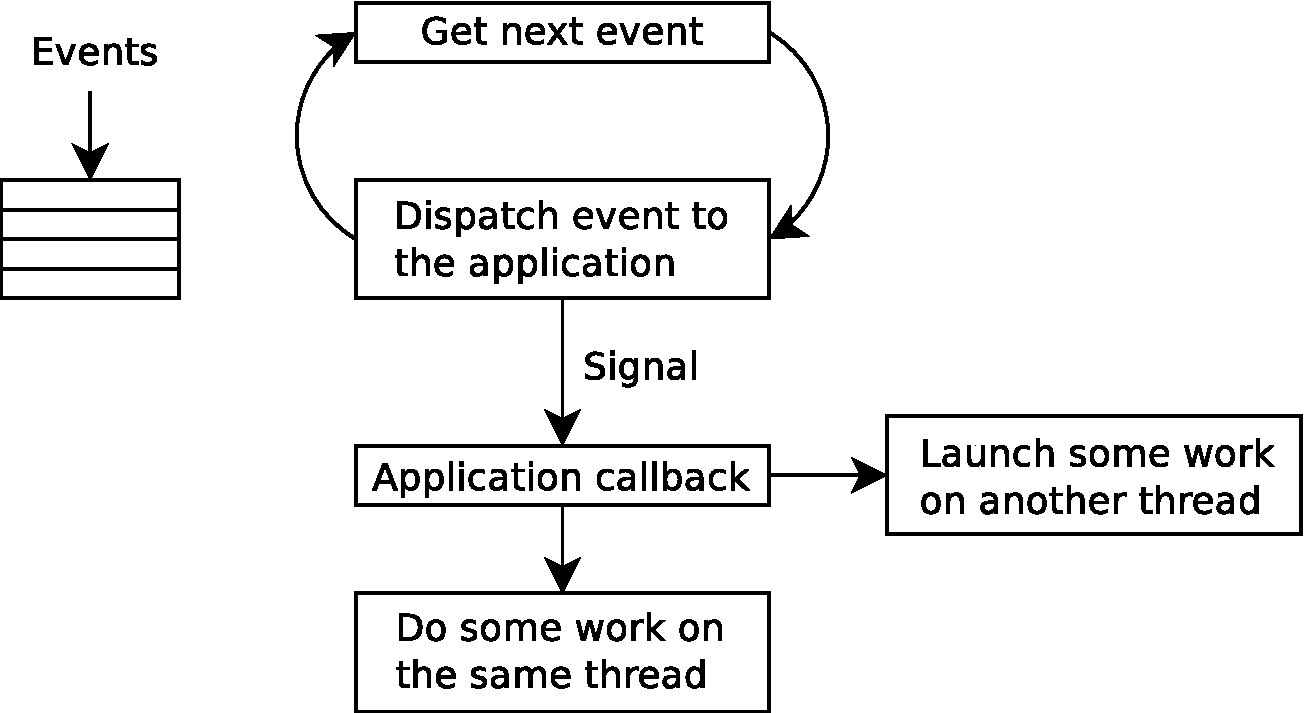
\includegraphics[width=10cm]{images/event-loop.pdf}
    \caption{Structure of an event-driven application, with a main event loop}
    \label{glib-event-loop}
  \end{center}
\end{figure}

Today's applications are often event-driven. For GUI applications, there are many sources of events: a key press, a mouse click, a touch gesture, a message from another application, a change on the file-system, being connected or disconnected from the network, and so on. An application needs to react to those events. For example when a key is pressed when a text entry has the focus, the character should be inserted and displayed on the screen.

But event-driven programming applies also to daemons. Inter-process communication also happens between daemons and applications. A daemon could receive an event when a packet arrives on a network interface. A printer daemon could receive events when a printer is connected, disconnected, is low-on-paper, etc. A mount daemon can listen to USB sticks inserted. Another daemon can listen to external monitors connections to reconfigure the screens, and so on.

An event-driven program is not structured the same as a batch program. The work to do by a batch program is determined at the start. It then analyzes the input, do some computations on it, and outputs a report. For instance, most Unix commands and scripts are batch programs.

So, how to structure an application that needs to respond to various events that can arrive at any time? As the title of this section suggests... with a \emph{main event loop} of course! That's another important part of GLib; it provides core support of event-driven programming, with a main event loop abstraction, a portable implementation of threads and asynchronous communication between threads. An event loop listens some sources of events. A priority is associated with each source of events. When an event arrives, the event loop dispatches it to the application. The event can then be taken into account, either in the same thread or another thread. The Figure~\ref{glib-event-loop} shows a high-level view of what is a main event loop.

The \lstinline{main()} function of an event-driven application looks like:
\begin{lstlisting}
gint
main (gint   argc,
      gchar *argv[])
{
  /* Create main window and attach signal callbacks. */

  /* Run the main event loop. */
  gtk_main ();

  return 0;
}
\end{lstlisting}

The GTK+ event loop is slightly higher level than the GLib event loop abstraction. \lstinline{gtk_main()} runs the main event loop until \lstinline{gtk_main_quit()} is called. \lstinline{gtk_main_quit()} is typically called in the function callback when the close button is clicked or the Quit menu action is activated.

A callback is a function that is called when a signal is sent. The signal system is implemented by the GObject library. Listening to a signal is achieved with the \lstinline{g_signal_connect()} function:
\begin{lstlisting}
static void
button_clicked_cb (GtkButton *button,
                   gpointer   user_data)
{
  MyObject *self = user_data;

  /* Do something */
}

static void
create_button (MyObject *self)
{
  GtkButton *button;

  /* Create button */

  /* Attach signal callback */
  g_signal_connect (button,
                    "clicked",
                    G_CALLBACK (button_clicked_cb),
                    self);
}
\end{lstlisting}

When a callback runs, it blocks the main loop. So to not freeze the user interface, there are two solutions:
\begin{enumerate}
  \item Long operations (especially I/O) can be launched in another thread.
  \item Long operations can be split into smaller chunks, and each chunk is run in a separate main loop iteration.
\end{enumerate}

For the second solution, GLib provides the \lstinline{g_idle_add()} and \lstinline{g_timeout_add()} functions (see Listing~\ref{glib-idle-timeout}). An idle function will be called when the main loop is idle, that is, when the main loop has nothing else to do. A timeout function is called at regular intervals. The boolean return value of a \lstinline{GSourceFunc} permits to continue or stop the function. If it continues, the function will be called again by the main loop, at the next idle time or timeout. You can manually remove the \lstinline{GSourceFunc} by calling \lstinline{g_source_remove()}, which takes as the parameter the source ID as returned by \lstinline{g_idle_add()} or \lstinline{g_timeout_add()}. You must pay attention to remove a \lstinline{GSourceFunc} when the object on which you do the computation is destroyed. So you can store the source ID in an object attribute, and call \lstinline{g_source_remove()} in the destructor if the source ID is different from \lstinline{0}. (See the GObject library to create your own classes in C.)

\begin{lstlisting}[float, caption={Idles and timeouts}, label=glib-idle-timeout]
#include <glib.h>

typedef gboolean (* GSourceFunc) (gpointer user_data);

guint g_idle_add (GSourceFunc function, gpointer data);
guint g_timeout_add (guint interval, GSourceFunc function, gpointer data);

gboolean g_source_remove (guint source_id);
\end{lstlisting}

\section{Other Features}

There simply isn't space to cover all of GLib's features in this book. It's worth looking at GLib whenever you find yourself thinking, ``There really \emph{should} be a function that...''. This section lists other features GLib provides, but is \emph{not} exhaustive.

Some core application support not already mentioned:
\begin{itemize}
  \item \lstinline{GError} -- an error reporting system, similar to exceptions in other languages.
  \item The \lstinline{g_log()} facility, allows you to print warnings, messages, etc. with configurable log levels and pluggable print routines.
\end{itemize}

Utilities:
\begin{itemize}
  \item A commandline option parser.
  \item A unit-test framework.
  \item A timer facility.
  \item Calendrical/date-arithmetic functions.
  \item Filename manipulation, such as \lstinline{g_path_get_basename()} and \lstinline{g_path_is_absolute()}.
  \item A simple XML parser.
  \item Perl-compatible regular expressions.
\end{itemize}

A selection of smaller utilities:
\begin{itemize}
  \item \lstinline{G_MAXFLOAT}, etc. equivalents for many numeric types.
  \item Byte-order conversions.
  \item \lstinline{G_DIR_SEPARATOR} handles Windows/Unix differences.
  \item Convenience/portability routines to get the user's home directory, get the name of a \texttt{/tmp} directory, and similar tasks.
  \item \lstinline{G_VA_COPY} copies a \lstinline{va_list} in a portable way.
  \item Numerous macros to permit the use of compiler extensions (especially GCC extensions) in a portable way.
  \item Bitfield manipulation.
  \item Portable \lstinline{g_htonl()} and other host-to-network conversions.
\end{itemize}

And last, but not least, other interesting data types:
\begin{itemize}
  \item Enhanced string and array classes. Pointer and byte arrays.
  \item \lstinline{GQuark} -- two way mapping from strings to integer identifiers.
  \item \lstinline{GVariant} -- a generic data type that stores a value along with information about the type of that value.
\end{itemize}
